\documentclass[aspectratio=43]{beamer}
\usetheme{Copenhagen}

% This is for handouts. uncomment if you want. put handout in document class
%\usepackage{pgfpages}
%\pgfpagesuselayout{4 on 1}[a4paper, border shrink=5mm, landscape]

\usepackage{amsmath}

\setbeamertemplate{navigation symbols}{}
\setbeamertemplate{headline}{}

\newcommand\blfootnote[1]{%
	\begingroup
	\renewcommand\thefootnote{}\footnote{#1}%
	\addtocounter{footnote}{-1}%
	\endgroup
}

\title{Academic Review - Physics}
\author{Dinan Mariano}
\institute{Institute of Mathematical Sciences and Physics \and University of the Philippines - Los Baños}
\date{January 2024}

\AtBeginSection[]{
	\begin{frame}
		\vfill
		\centering
		\begin{beamercolorbox}[sep=8pt,center,shadow=true,rounded=true]{title}
			\usebeamerfont{title}\insertsectionhead\par%
		\end{beamercolorbox}
		\vfill
	\end{frame}
}


\begin{document}
	
	
\begin{frame}[plain]
    \maketitle
\end{frame}

\begin{frame}{Topics}
	\tableofcontents

\end{frame}

\begin{frame}{Nobel and Ig Nobel Prizes}
	2023 Nobel Prize of Physics - for experimental methods that generate attosecond pulses of light for the study of electron dynamics in matter\\~\\
	\uncover<2-> {
	\begin{block}{Ig Nobel Prize}
		Honor "achievements that first make people laugh and then make them think."
	\end{block}}
	
	\uncover<3>{2023 Ig Nobel Prize of Education - for methodically studying the boredom of teachers and students}
\end{frame}

\section{Scalar and Vector}

\subsection{Scalar and Vector}

\begin{frame}
	\begin{columns}
		\column{0.5\textwidth} \textbf{Scalar Quantity} - a quantity which is expressed by magnitude only \\
		\begin{example}
			Mass \\
			Time \\
			Temperature \\
			Area \\
			Distance 
		\end{example}
		\column{0.5\textwidth} \textbf{Vector Quantity} - a quantity which is expressed by magnitude and direction \\
		\begin{example}
			Force \\
			Velocity \\
			Weight \\
			Acceleration \\
			Displacement
		\end{example}
	\end{columns}
\end{frame}

\begin{frame}{Quiz}
		
		\begin{columns}
			\column{0.3\textwidth}
			\begin{itemize}
				\item 5 m 
				\item 30 m/sec, East
				\item 5 km, North
				\item 20 degrees Celcius
				\item 1 GB
				\item 4000 calories
			\end{itemize}
			\column{0.7\textwidth}
			\begin{itemize}
				\item[--]<2-> Scalar
				\item[--]<3-> Vector
				\item[--]<4-> Vector
				\item[--]<5-> Scalar
				\item[--]<6-> Scalar
				\item[--]<7-> Scalar
			\end{itemize}
		\end{columns}
\end{frame}

\subsection{Resultant Vector}

\begin{frame}
	\textbf{Resultant Vector}
	\begin{definition}
		Sum of two or more vectors which will give the same effect as the original vectors
	\end{definition}
\end{frame}


\begin{frame}{Process of finding the Resultant Vector}
	
	\begin{enumerate}
		\item Addition/Subtraction
		\item Pythagorean Theorem
		\item Component Method
	\end{enumerate}
	
\end{frame}

\begin{frame}{Addition/Subtraction}
	\begin{columns}
		\column{0.5\textwidth}
		Can only be used on 1D vectors \\ (same direction)\\~\\
		\uncover<2-> {What if we encounter more complicated vectors?\\
		\begin{center}
			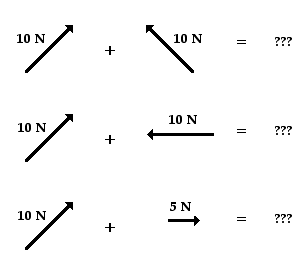
\includegraphics[scale=0.4]{compvec.png}
		\end{center}}
		\column{0.5\textwidth}
		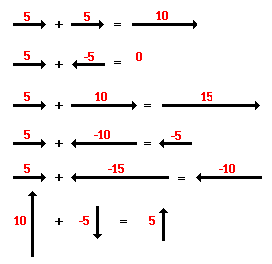
\includegraphics[scale=0.5]{vectoradd.png}
	\end{columns}
	\blfootnote{Images from www.physicsclassroom.com}
\end{frame}

\begin{frame}{Pythagorean Theorem}
	\begin{block}{Pythagorean Theorem}
		$ a^2 + b^2 = c^2$
	\end{block}
	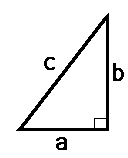
\includegraphics[scale=0.3]{pytha.png}  \uncover<2>{\alert{only use pythagorean theorem on perpendicular vectors!}}\\
	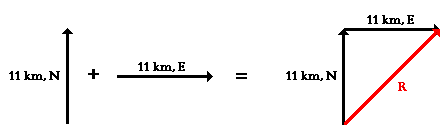
\includegraphics[scale=0.3]{pythaexample.png}
	\centering 
	\begin{align*}
		11^2 + 11^2 &= R^2\\
		242 &= R^2\\
		15.6 &= R
	\end{align*}
	\blfootnote{Images from www.physicsclassroom.com}
\end{frame}

\begin{frame}{Component Method}
	\begin{example}
		An airplane flies in a northeasterly direction at 100 km/h, at the same time there is a wind blowing at 20 km/h to the northwest. What is the resultant velocity of the plane?
	\end{example}
	X-components:
	\begin{align*}
		V_{xplane} &= V_{plane} \cos 45^\circ \\
		&= 70.71 \text{ km/h}	\\
		V_{xwind} &= -V_{wind}  \cos 45^\circ \\
		&= -14.14 \text{ km/h}
	\end{align*}
	\blfootnote{$V_{xwind}$ can be equal to $V_{wind} \cos 135^\circ$ with the same answer}
\end{frame}

\begin{frame}{Component Method (cont.)}
	Y-compoments:
	\begin{align*}
		V_{yplane} &= V_{plane} \sin 45^\circ \\
		&= 70.71 \text{ km/h} \\
		V_{ywind} &= V_{wind}  \sin 45^\circ \\
		&= 14.14 \text{ km/h}
	\end{align*}

\end{frame}

\begin{frame}{Component Method (cont.)}

	Resultant Velocity
	\begin{align*}
		V_x &= V_{xplane} + V_{xwind} \\
		&= 70.71 - 14.14 \\
		& = 56.57 \text{ km/h} \\
		V_y &= V_{yplane} + V_{ywind} \\
		&= 70.71 + 14.14 \\
		&= 84.85 \text{ km/h}\\
		R &= \sqrt{56.57^2 + 84.85^2} \\
		R &= 101.978857613  \text{ km/h}\\
		\theta &= \arctan{\frac{84.85}{56.57}} \\
		\theta &= 56.31^\circ
	\end{align*}
\end{frame}

\section{Mechanics}

\begin{frame}{Motion}
	\begin{definition}
		Change in position of a object relative to other objects that are considered at rest
	\end{definition}
	
\end{frame}


\section{Newton's Law of Motion}

\section{Momentum and Impulse}

\section{Work, Energy, and Power}

\end{document}
